\documentclass{ecnreport}
%
\stud{Option Robotique, Control \& Robotics master}
\topic{Advanced Programming}

\begin{document}

\inserttitle{Advanced Programming}
\insertsubtitle{Solving Sudokus}

\section{Context}

Sudoku is a popular game that is played on a $9\times$ 9 grid, some cells containing digits between 1 and 9 and some empty.
Playing the game amounts to filling the grid with only 4 rules:
\begin{itemize}
 \item Each cell should have a digit between 1 and 9
 \item Each row should contain all digits
 \item Each column should contain all digits
 \item Each of the 9 sub-square of dimension $3\times 3$ should contain all digits
\end{itemize}

The difficulty of a Sudoku represents how many candidates exist in each empty cell at the beginning. An easy Sudoku will contain some cells having only one candidate, leading to a sure guess. A difficult Sudoku will contain only cells having several candidates, forcing the player to rely on hypotheses until a contradiction occurs.


\begin{figure}[h!]\centering
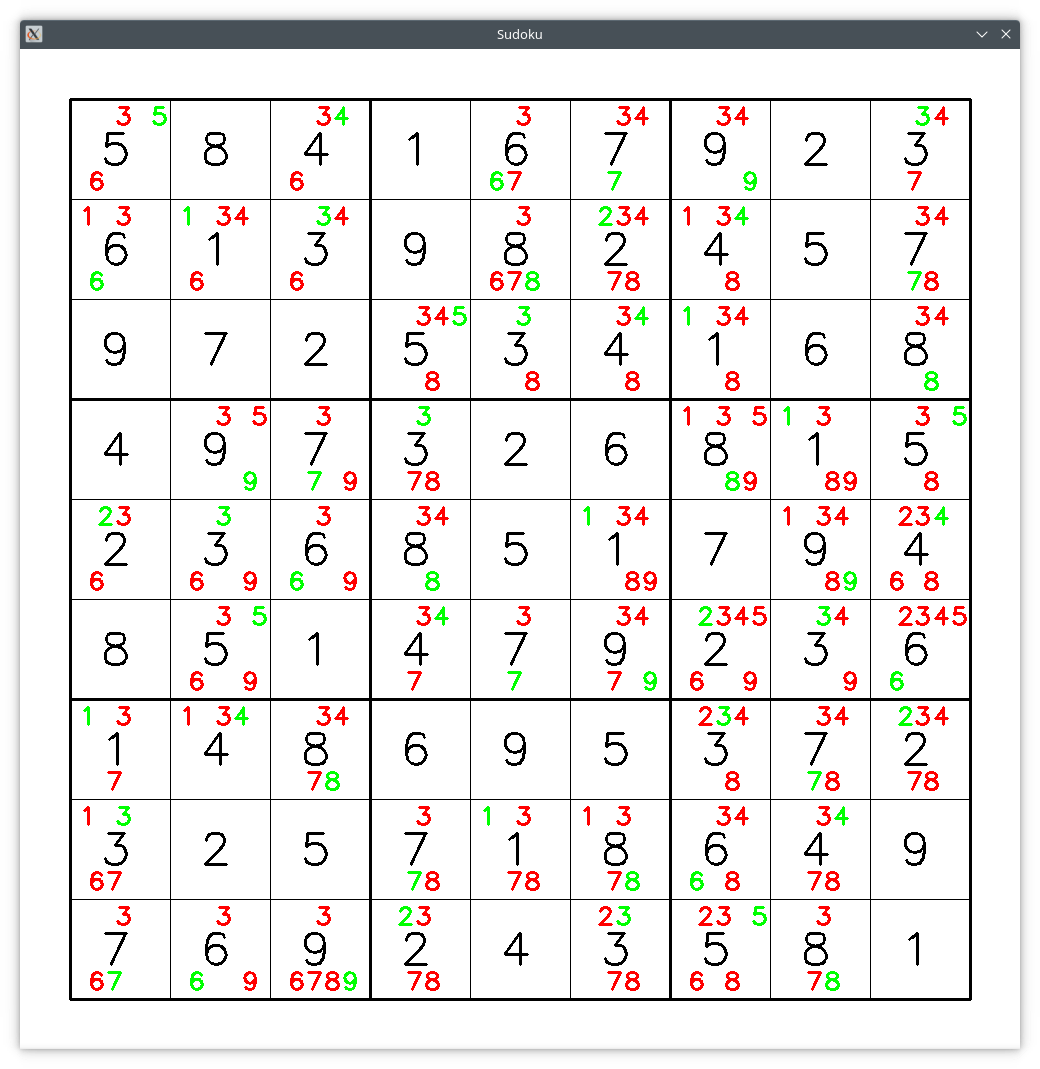
\includegraphics[width=.5\linewidth]{sudoku.png}
\caption{A solved Sudoku. Red digits show initial candidates for each cell. Green digits are the initial candidate that was the valid one at the end. Cells without red/green digits are the ones from the starting grid.}
\label{fig:trilat}
\end{figure}

\section{Backtracking algorithm}

Backtracking is a simple algorithm that can solve Sudoku quite well. It solves the cells one at the time, possibly doing a guess among the candidate digits. If it finds a contradiction, is cancels the previous guess and tries the next one. For an easy Sudoku, this algorithm will never have to do any wild guess and will solve the grid without ever cancelling a guess.\\
\newcommand{\var}[1]{\texttt{\upshape #1}}

The algorithm reads as follows, under the \var{solveNextCell()} function.\\
This function is recursive as once a guess is done on a cell, it calls \var{solveNextCell()} again.

 \begin{algorithm}[!h]
 \DontPrintSemicolon
 \SetKwFunction{Fill}{{\bf Function} solveNextCell}\;
 \Fill{}
 {
 \\
 \If{\var{grid} is full}{\Return \var{true}\;}
\var{next\_cell} $\gets$ best next cell to investigate\;
\For{\var{guess} in \var{next\_cell.candidates}}{
 \tcp{let's assume this guess is the correct one}
Assign \var{guess} to \var{next\_cell} \tcp{also prune from \var{neighboors}}
\If{\var{solveNextCell()}}{\Return \var{true}\; }
\tcp{\var{guess} leads to some contradiction}
Cancel \var{guess} for \var{next\_cell} \tcp{also restore it from \var{neighboors} that had it}
}
\tcp{We have tried all candidates for this cell, without success}
\Return \var{false}\;
}
% \SetAlgoLined

\caption{Backtracking algorithm}
\label{backtracking}
\end{algorithm}

As we can see the algorithm relies on a few underlying functions, that are expressed as methods (member functions) of the \okt{Cell} class:

\begin{itemize}
 \item A \okt{Cell} should be able to tell if a given guess could be set as its digit
 \item A \okt{Cell} should be able to set a guess and prune it from its neighboors
 \item A \okt{Cell} should be able to cancel a guess and restore it for its neighboors
\end{itemize}

Additionally, a grid should be able to tell if it is full, that is all its cells have a digit.

\newpage
\section{Available classes and methods to implement}

\def\Grid{\okt{Grid}~}
\def\Cell{\okt{Cell}~}

The \okt{main} function is quite trivial and only loads the desired Sudoku to solve. The algorithm itself is done through two classes: \Grid and \Cell.

\subsection{\Grid class}

The \Grid class has:
\begin{itemize}
 \item An array of 81 \Cell called \okt{cells}
 \item A constructor that takes a starting grid and should initialize the \okt{cells} accordingly
 \item A \okt{solve()} method that enters the solving process and prints the outcome
 \item A \okt{solveNextCell()} method that implements the backtracking algorithm
\end{itemize}

You have to implement:
\begin{itemize}
 \item the constructor that initializes the starting grid but does not yet erase candidate values for neighboors of cells defined in the grid
 \item the \okt{solveNextCell()} method (shown in Algorithm \ref{backtracking})
\end{itemize}

\subsection{\Cell class}

As seen above, most of the intelligence comes from the cell being able to change its guess and inform its neighboors.
The \Cell class has:
\begin{itemize}
 \item A \okt{init} function that takes the row and column of the cell, the whole \okt{cells} array from the grid and any initial value this cell should have
 \item A \okt{uint} called \okt{digit_} that is the current guess for this cell. If \okt{digit_} is 0 it means this cell was not assigned a value at this point of the algorithm
 \item A vector of \okt{uint} called \okt{candidates_} that lists the remaining candidates at any point during the algorithm
 \item An array of \okt{uint} called \okt{pruned_} that tells how many times a given digit was pruned for this cell. Index 0 is not used so for example \okt{pruned_[3]} tells how many times 3 was said to be a forbidden value for this cell
 \item An array of 20 pointers to \Cell called \okt{neighboors_} that point to all other cells that cannot have the same digit as this one
 \item 2 member functions to deal with the candidates: \okt{eraseCandidate(guess)} and \okt{hasCandidate(guess)}
 \item A static functions \okt{isValid(cell)} to be used in algorithms
 \item 2 member functions that are called by the backtracking algorithm: \okt{set(guess)} and \okt{cancel()}
 \item 2 member functions that keeps track of guesses in connected cells: \okt{prune(guess)} and \okt{restore(guess)}
\end{itemize}

\fbox{You have to implement these four last methods, their definition being listed below}

\paragraph{\bf \okt{void prune(uint guess)}}~\\

 \begin{minipage}{.5cm}
~
 \end{minipage}
 \begin{minipage}{0.9\linewidth}
    This method should delete the given guess from the candidates of this cell, if these two conditions are met:

\begin{itemize}
 \item The cell does not have a digit yet
 \item The guess to be pruned is actually in the candidates, or the guess was already pruned
\end{itemize}

If the guess is actually in the candidates, it should be removed. In any case the corresponding value in the \okt{pruned} array should be incremented to keep track how many times this was pruned.
 \end{minipage}




\paragraph{\okt{void restore(uint guess)}}~\\

 \begin{minipage}{.5cm}
~
 \end{minipage}
 \begin{minipage}{0.9\linewidth}
This method should decrement the pruning counter of the given guess for this cell:

\begin{itemize}
 \item The cell does not have a digit yet
 \item The guess was indeed pruned
\end{itemize}
If both these conditions are true, the counter in \okt{pruned_} should be decremented. If this counter falls back to 0, the guess should be added again to the \okt{candidates}.
 \end{minipage}


 \paragraph{\okt{void set(uint guess)}}~\\

 \begin{minipage}{.5cm}
~
 \end{minipage}
 \begin{minipage}{0.9\linewidth}
This method should set the guess on this cell and prune it from its neighboors
 \end{minipage}

  \paragraph{\okt{void cancel()}}~\\

 \begin{minipage}{.5cm}
~
 \end{minipage}
 \begin{minipage}{0.9\linewidth}
This method should cancel the current guess on this cell (available in \okt{digit_}) and restore it from its neighboors
 \end{minipage}

 \subsection{Tips}

 All the methods can be written in a few lines by using modern C++ that is:
 \begin{itemize}
  \item range-based for loops
  \item \okt{<algorithm>} functions such as \okt{std::any\_of} and \okt{std::all\_of}, possibly with lambda or existing functions
 \end{itemize}

 Some basic errors will lead to the program crashing, {\bf use the debugger} to understand what went wrong.
\\
You can also use it with breakpoints to see what is going on in this mess.\\

Do not modify parts of the code you are not supposed to implement or you will never be able to solve a Sudoku again.


\newpage


\subsection{Bonus: improve the \okt{bestNextCell} function}

In \okt{grid.cpp} the \okt{bestNextCell} function takes two \Cell called \okt{c1, c2} and returns whether \okt{c1} should be investigated before \okt{c2}. The initial function just compares the cells' digit, ensuring that a cell with digit 0 (e.g. no guess yet) will always be chosen over a cell that is already set.

This may lead the algorithm to start with cells that have a large number of candidates, while some others may have less and even only one. Improve this function as you think is best and compare the solving times.

\subsection{Bonus: keep track of the algorithm back and forth}

The \Grid class has member variables called \okt{guesses} and \okt{cancels} that are printed at the end. Update them in the \okt{solveNextCell} function to see what happens under the hood.


\section{Starting grids}

The \okt{starts} folder lists several starting grids, to be set in the \okt{main} function to test your algorithm:
\begin{itemize}
 \item \okt{basic0} is already filled. You should start with that to test the exit criterion.
 \item \okt{basic1} and \okt{basic2} have respectively only 1 and 2 empty cells
 \item \okt{easy}, \okt{medium}, \okt{hard} and \okt{harder} are of increasing complexity
\end{itemize}



\end{document}
